\section{Lab 1: Triển khai Mô hình Mạng Phẳng (Flat Network)}

\subsection{Kiến trúc Tổng quan và Phân bổ Tài nguyên}
Mô hình mạng phẳng (Flat Network) là kiến trúc mạng nguyên thủy nhất, trong đó toàn bộ Campus được đặt trong một miền quảng bá (Broadcast Domain) khổng lồ ở Layer 2. Thiết kế này không có sự phân chia logic (VLAN) giữa các khu vực Hành chính, Lab, hay Ký túc xá.

\begin{figure}[H]
    \centering
    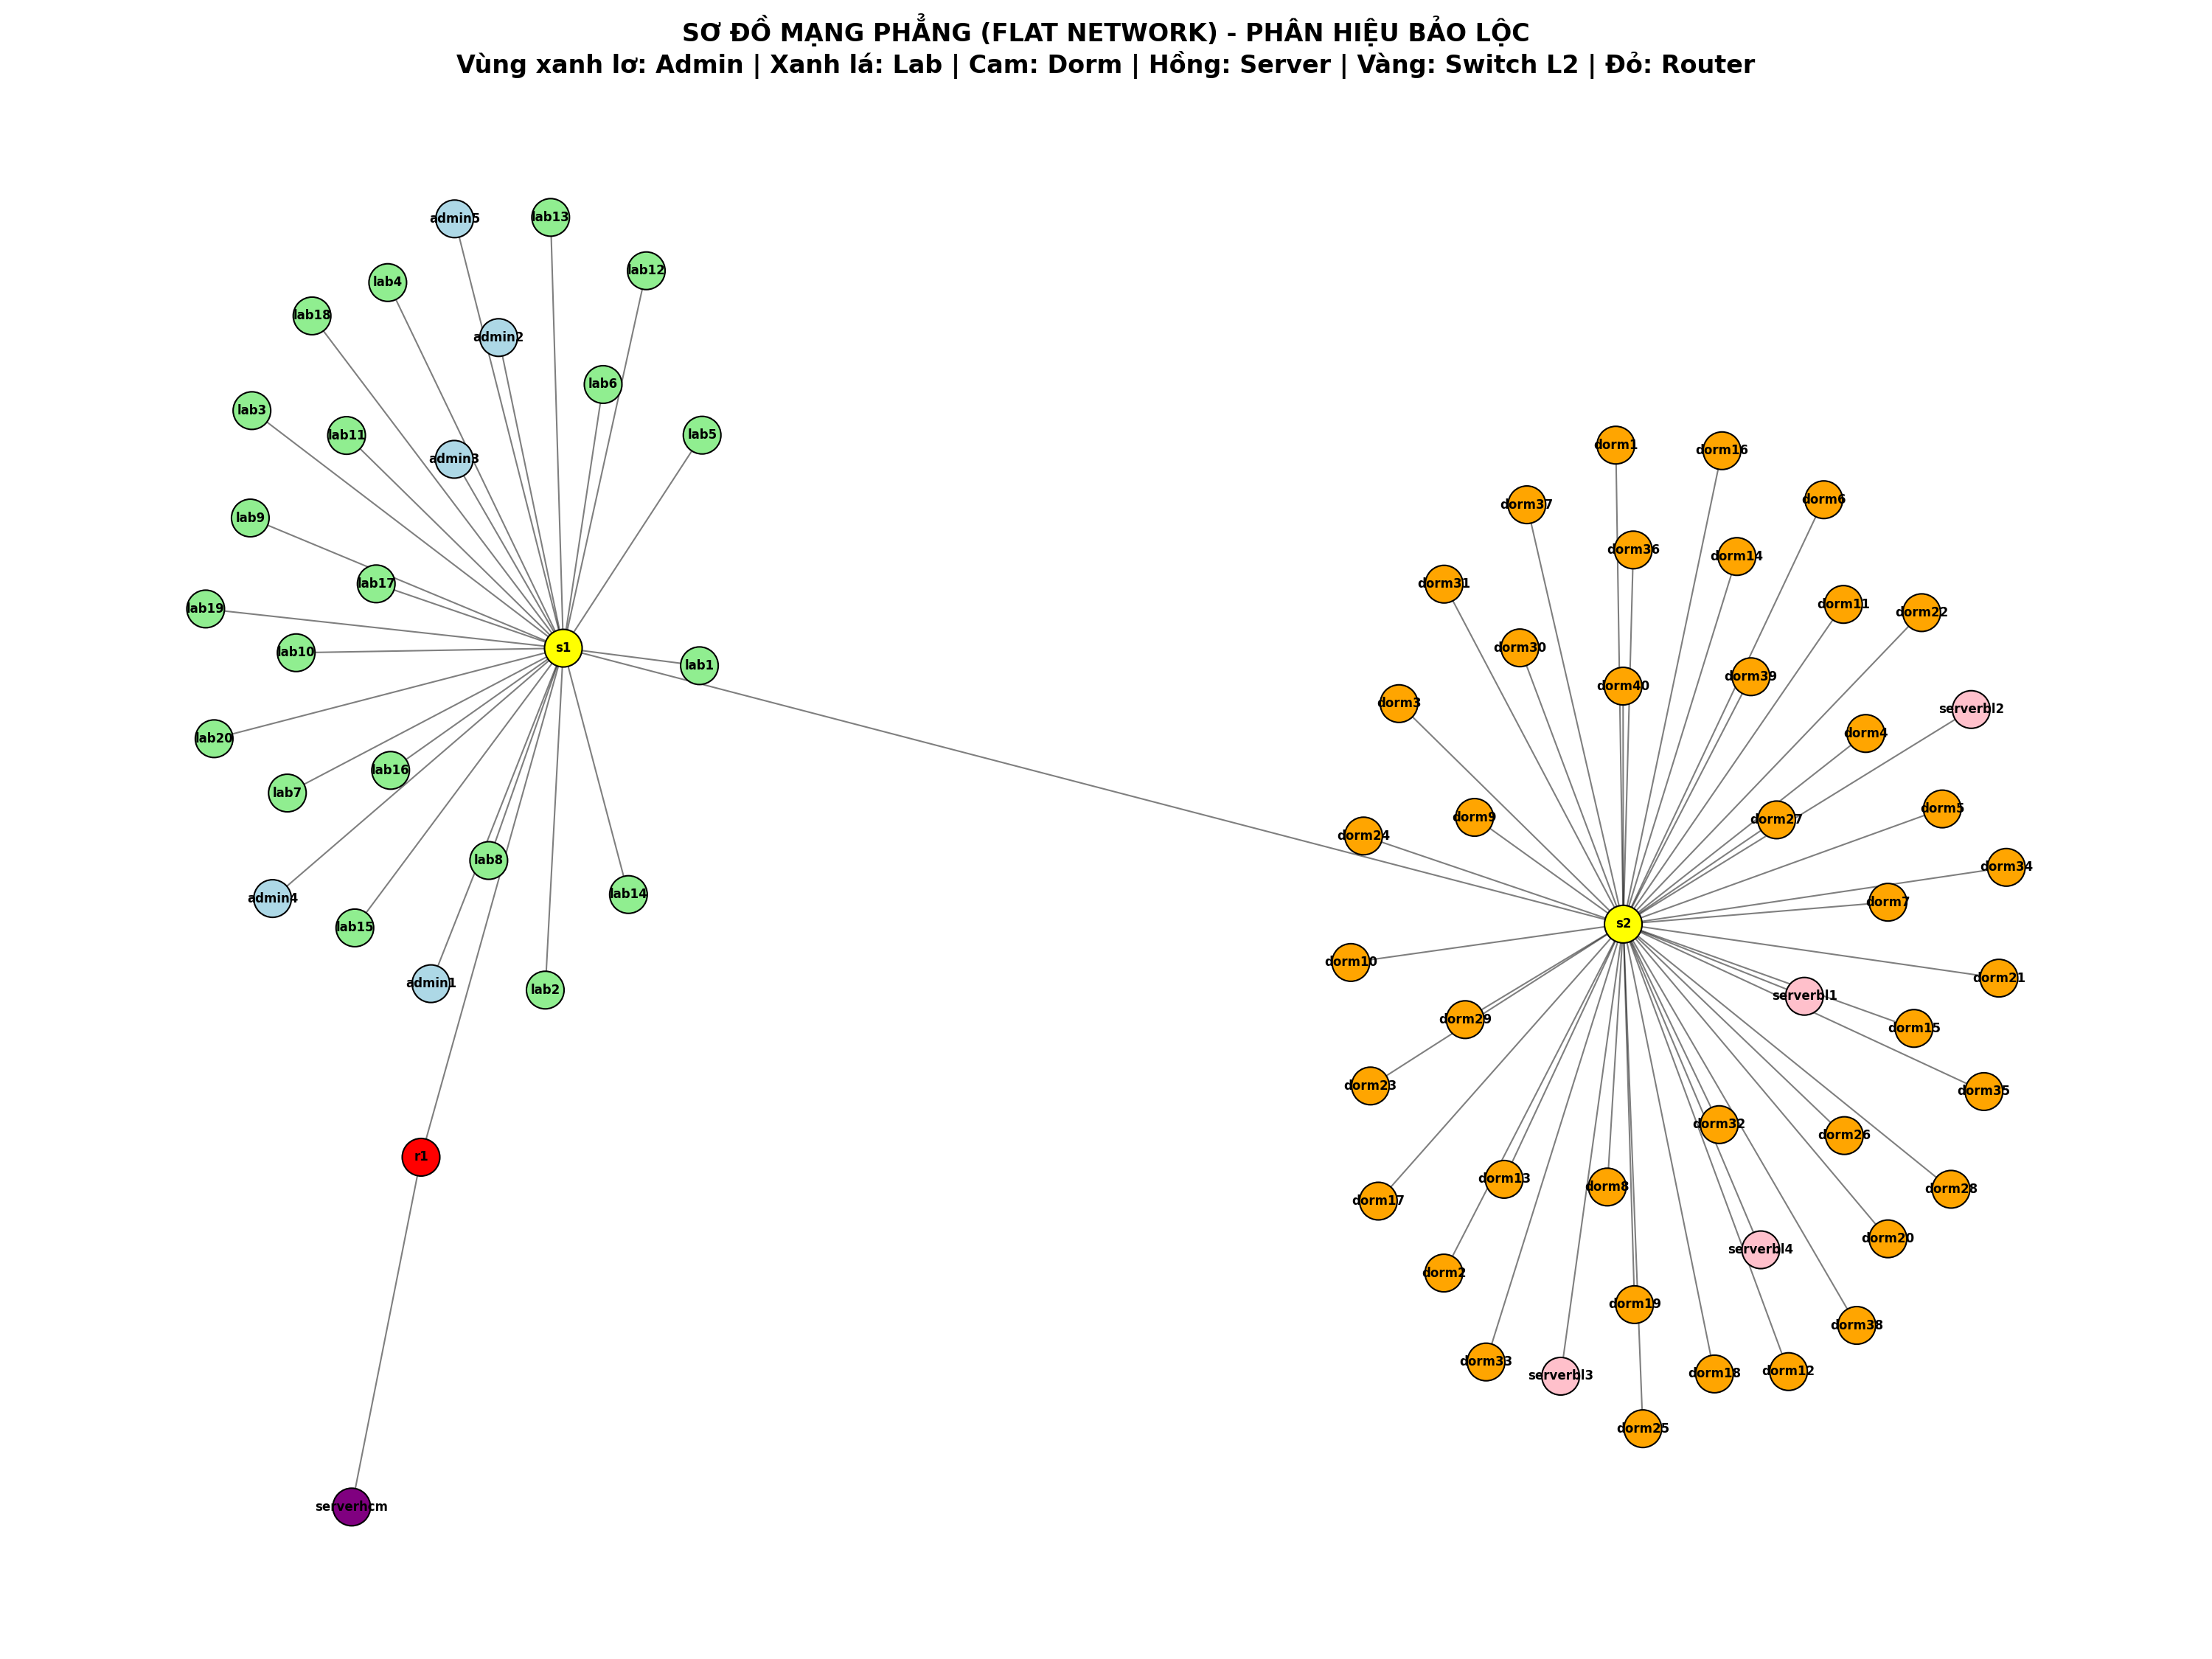
\includegraphics[width=0.8\linewidth]{image/topology_mohinh1.png}
    \caption{Sơ đồ kiến trúc mạng phẳng (Flat Network) tại Phân hiệu Bảo Lộc}
    \label{fig:mh1_topo}
\end{figure}

\subsection{Quy hoạch Không gian IP và Định tuyến Biên}
Toàn bộ 69 thiết bị đầu cuối trong hệ thống được quy hoạch sử dụng chung một dải mạng Subnet lớn: \texttt{10.0.0.0/16}.

Việc cấp phát IP logic được chia theo từng vùng để dễ quản lý:
\begin{itemize}
    \item Vùng Admin (Ban Giám Hiệu - 5 hosts): dải IP \texttt{10.0.1.x}
    \item Vùng Lab AI (20 hosts): dải IP \texttt{10.0.2.x}
    \item Vùng Ký túc xá (40 hosts): dải IP \texttt{10.0.3.x}
    \item Vùng Server Local (4 hosts): dải IP \texttt{10.0.4.x}
\end{itemize}

Về định tuyến biên (Edge Routing), hệ thống triển khai một Edge Router làm Default Gateway tại IP \texttt{10.0.0.254}. Cổng WAN của Router này đóng vai trò kết nối với Server HCM (\texttt{203.162.1.1}) thông qua đường link bị giới hạn băng thông 200 Mbps.

\subsection{Quy tắc Đặt tên \& Giới hạn Thiết bị}
Khi thiết lập mô hình trên Mininet, bắt buộc phải tuân thủ các quy định sau:
\begin{itemize}
    \item Mỗi switch chỉ kết nối được tối đa 48 host.
    \item Quy tắc đặt tên switch: \texttt{s1}, \texttt{s2}, \dots
    \item Quy tắc đặt tên router: \texttt{r1}, \texttt{r2}, \dots
    \item Quy tắc đặt tên host: \texttt{admin1}, \texttt{admin2}, \dots, \texttt{serverhcm}, \texttt{serverbl1}, \texttt{lab1}, \dots, \texttt{dorm1}, \dots
\end{itemize}

Phân bổ băng thông kết nối vật lý:
\begin{itemize}
    \item 5 máy Admin $\leftrightarrow$ Core Switch: 100 Mbps
    \item 20 máy Lab AI $\leftrightarrow$ Core Switch: 1 Gbps
    \item 40 máy Ký túc xá $\leftrightarrow$ Core Switch: 50 Mbps
    \item 4 máy Server Local $\leftrightarrow$ Core Switch: 1 Gbps
    \item Cổng LAN Edge Router $\leftrightarrow$ Core Switch: 1 Gbps
    \item Cổng WAN Edge Router $\leftrightarrow$ Server HCM: 200 Mbps, độ trễ 10ms
\end{itemize}

\subsection{Quy trình Triển khai Top-Down}

\subsubsection{Bước 1: Cấu hình trên Edge Router (Gateway)}
\begin{itemize}
    \item Kích hoạt IP Forwarding: \texttt{sysctl -w net.ipv4.ip\_forward=1}
    \item Cấu hình cổng LAN (Inside): IP \texttt{10.0.0.254/16}
    \item Cấu hình cổng WAN (Outside): IP \texttt{203.162.1.254/24}
    \item Bảng định tuyến tự động biết các mạng trực tiếp kết nối.
\end{itemize}

\subsubsection{Bước 2: Cấu hình trên Core Switch (Switch L2)}
\begin{itemize}
    \item Không cần cấu hình (Zero Configuration).
    \item Switch hoạt động ở chế độ Plug-and-Play: tự động học MAC và chuyển tiếp frame.
    \item Mọi gói broadcast (bao gồm ARP) sẽ được nhân bản ra toàn bộ cổng.
\end{itemize}

\subsubsection{Bước 3: Cấu hình trên 69 Hosts Nội bộ}
\begin{itemize}
    \item Gán IP theo vùng nhưng sử dụng chung Subnet Mask \texttt{/16} (255.255.0.0).
    \item Trỏ Default Gateway về \texttt{10.0.0.254} trên tất cả host:
    \begin{verbatim}
    ip route add default via 10.0.0.254
    \end{verbatim}
\end{itemize}

\subsubsection{Bước 4: Cấu hình Server HCM (Đầu xa)}
\begin{itemize}
    \item Gán IP: \texttt{203.162.1.1/24}
    \item Thêm định tuyến ngược:
    \begin{verbatim}
    ip route add 10.0.0.0/16 via 203.162.1.254
    \end{verbatim}
\end{itemize}

\subsection{Thao tác Thực thi trong Môi trường Ubuntu Linux}

\subsubsection{Dọn dẹp \& Chuẩn bị Môi trường}
\begin{lstlisting}[language=bash]
# Kiem tra thu muc hien tai
pwd

# Xoa mo hinh mininet cu
sudo mn -c

# Buoc dung tien trinh neu can
sudo killall -9 mininet 2>/dev/null
\end{lstlisting}

\subsubsection{Khởi chạy File Kịch bản Python}
\begin{lstlisting}[language=bash]
sudo python3 cauhinh1.py
\end{lstlisting}
Sau khi chạy thành công, giao diện chuyển sang prompt \texttt{mininet>}.

\begin{figure}[H]
    \centering
    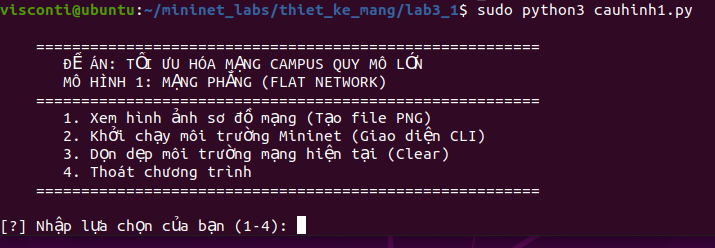
\includegraphics[width=0.8\linewidth]{image/mininet_start.png}
    \caption{Khởi chạy thành công môi trường Mininet và hội tụ IP}
    \label{fig:mh1_start}
\end{figure}

\subsection{Các Kịch bản Kiểm thử Hiệu năng}

\subsubsection{Bài Test 1: Đo lường Băng thông East-West (Elephant Flow)}
Mục đích: Kiểm tra hiện tượng nghẽn cổ chai tại Core Switch khi có luồng dữ liệu lớn trao đổi nội bộ giữa khu vực Lab và Server.
\begin{lstlisting}[language=bash]
# Tren giao dien Mininet, mo cong lang nghe iperf tren serverbl1
mininet> serverbl1 iperf -s &

# Day luong du lieu tu lab1 den serverbl1 trong 10 giay
mininet> lab1 iperf -c 10.0.4.1 -t 10
\end{lstlisting}

\begin{figure}[H]
    \centering
    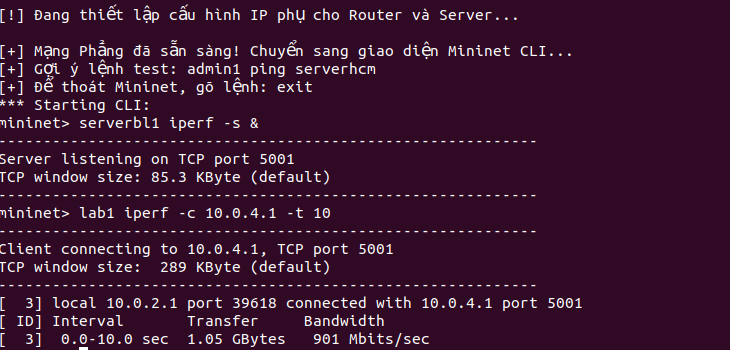
\includegraphics[width=0.8\linewidth]{image/iperf_test1.png}
    \caption{Kết quả đo đạc băng thông iperf giữa Lab và Server}
    \label{fig:iperf_test1}
\end{figure}

\subsubsection{Bài Test 2: Nghẽn mạng WAN (Oversubscription)}
Mục đích: Quan sát tỷ lệ rớt gói và độ trễ của mạng Hành chính (Admin) khi băng thông WAN bị Ký túc xá (Dorm) vắt kiệt.
\begin{lstlisting}[language=bash]
# Tao may chu UDP tren serverhcm (Dau xa)
mininet> serverhcm iperf -s -u &

# Tao luong traffic lon (250Mbps) tu Dorm day ra WAN
mininet> dorm1 iperf -c 203.162.1.1 -u -b 250M -t 15 &

# Cung luc do, kiem tra do tre tu Admin
mininet> admin1 ping -c 10 203.162.1.1
\end{lstlisting}
\textbf{Đánh giá kết quả:} Lệnh ping trả về độ trễ cực cao hoặc thông báo \texttt{Destination Host Unreachable}. Điều này minh chứng mạng phẳng không có khả năng kiểm soát luồng (QoS).

\begin{figure}[H]
    \centering
    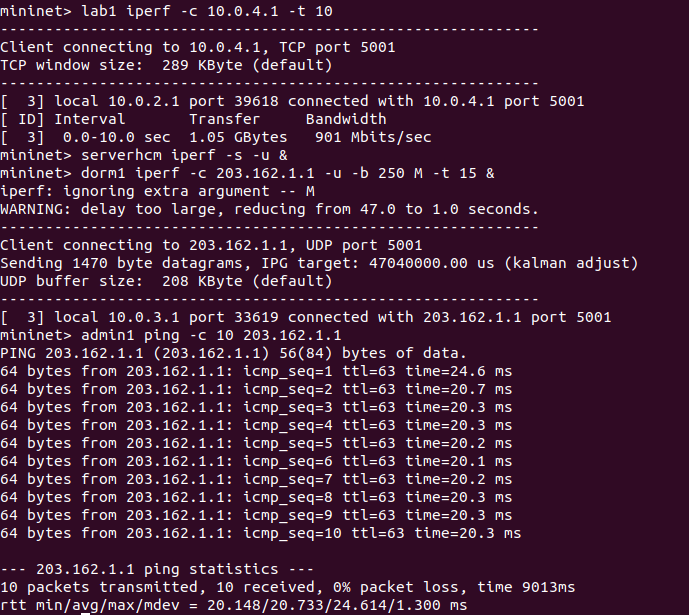
\includegraphics[width=0.8\linewidth]{image/ping_test2.png}
    \caption{Độ trễ và rớt gói của Admin khi đường WAN quá tải}
    \label{fig:ping_test2}
\end{figure}

\subsubsection{Bài Test Mở rộng: Tấn công Tràn bảng MAC (MAC Flooding)}
Mục đích: Phơi bày sự mong manh của mạng phẳng khi bị tấn công tràn bảng MAC (CAM Table Overflow).
\begin{lstlisting}[language=bash]
# Mo hai cua so xterm rieng biet
mininet> xterm dorm1 admin1

# Tren cua so admin1, chay ping lien tuc den Server Local
root@admin1:~# ping 10.0.4.1

# Tren cua so dorm1, kich hoat MAC flooding
root@dorm1:~# macof -i dorm1-eth0
\end{lstlisting}
\textbf{Phân tích:} Bảng MAC của Core Switch bị quá tải $\rightarrow$ Switch rơi vào trạng thái giống Hub $\rightarrow$ mọi frame đều bị flood $\rightarrow$ nghẽn nghiêm trọng toàn mạng.

\subsection{Khắc phục Sự cố Thường gặp}
\begin{itemize}
    \item Lệnh \texttt{macof} không tồn tại $\rightarrow$ Cài đặt gói: \texttt{sudo apt-get install dsniff}
    \item Ping ra Server HCM báo Network Unreachable $\rightarrow$ Kiểm tra đã bật \texttt{ip\_forward=1} trên \texttt{r1} chưa.
    \item Log OVS báo đầy bộ nhớ $\rightarrow$ Đây là hiện tượng bình thường khi chạy MAC flooding.
\end{itemize}